\documentclass[12pt]{article}

\usepackage{amsmath, amssymb, amsthm}
\usepackage{geometry}
\usepackage{graphicx}
\usepackage{tikz}
\usepackage{hyperref}

\geometry{margin=1in}

% Theorem environments
\newtheorem{theorem}{Theorem}[section]
\newtheorem{lemma}[theorem]{Lemma}
\newtheorem{proposition}[theorem]{Proposition}
\newtheorem{corollary}[theorem]{Corollary}
\theoremstyle{definition}
\newtheorem{definition}[theorem]{Definition}
\newtheorem{example}[theorem]{Example}
\theoremstyle{remark}
\newtheorem{remark}[theorem]{Remark}

% Notation shortcuts
\newcommand{\ZZ}{\mathbb{Z}}
\newcommand{\St}{\mathrm{St}}
\newcommand{\kpoly}{k}

\title{The Structural Polynomial of a Parity Sequence\\
and Its Applications}

\author{Jon Seymour\\
  \texttt{jon@wildducktheories.com}\\
  Sydney, Australia}
\date{July 2026}

\begin{document}

\maketitle

\begin{abstract}
We develop a polynomial representation for parity sequences of generalised
Collatz-type maps $(g,h,q)$, working in the ring $\ZZ[g,h]$ rather than
specialising immediately to numerical values.  The central object is the
\emph{structural polynomial} $\kpoly_w(g,h)$ attached to a parity sequence,
which encodes the accumulated additive contribution of the odd steps
independently of the parameter $q$.

The main results are: (1) a \emph{path identity} $h^e b = g^o a + q\kpoly_w(g,h)$
valid for any parity sequence; (2) a \emph{geometric polynomial theorem} showing
that Steiner words $\St(\alpha,\beta)$ have $\kpoly(g,h) = (g^\alpha -
h^\alpha)/(g-h)$, independent of $\beta$; (3) a \emph{composition rule}
$\kpoly_{Q\circ P} = g^{o_Q}\kpoly_P + h^{e_P}\kpoly_Q$; and (4) a
\emph{cycle element identity} $a = q\kpoly_w/(h^e - g^o)$ giving the fixed
point as a rational function of $(g,h,q)$.

Beyond these core results, we develop a system of five equivalent
representations of any parity sequence --- its bits (the $p$-value), the
structural polynomial $\kpoly_w(g,h)$, its specialisation $\kpoly_w(3,2)$,
the $\sigma$-polynomial $\sigma_w(u,v)$, and the Collatz orbit $\phi_w$ ---
connected by explicitly invertible transformations.  We also introduce a
successor operation on $\kpoly_w$ in $\ZZ/(h^e-g^o)\ZZ$ that generates all
cycle representatives by rotation, and we warn that polynomial
non-divisibility of $h^e - g^o \nmid \kpoly_w$ in $\ZZ[g,h]$ does not
preclude pointwise divisibility at specific integer bases.
Applications to the $2a+1$ composition identity are developed in the companion
paper~\cite{paper73}.
\end{abstract}

\tableofcontents

\bigskip

%------------------------------------------------------------
\section{Introduction}
\label{sec:intro}
%------------------------------------------------------------

A \emph{generalised Collatz-type map} with basis $(g,h,q)$ consists of two
elementary operations on the positive integers: an \emph{odd step}
$x \mapsto gx + q$ and an \emph{even step} $x \mapsto x/h$.  The standard
Collatz map (the Syracuse odd-only iteration) uses basis $(g,h,q) = (3,2,1)$;
the $5x+1$ analogue uses $(5,2,1)$.  A \emph{parity sequence} is a finite
word over $\{O, E\}$ specifying the order in which these steps are applied.
Each parity sequence acts as an affine map on its domain of definition.

The central algebraic object we study is the \emph{structural polynomial}
$\kpoly(g,h) \in \ZZ[g,h]$ attached to a parity sequence.  It captures the
additive part of the parity sequence's affine action in a basis-independent
form.  The key advantage of working in $\ZZ[g,h]$ rather than substituting
$g = 3$, $h = 2$ at the outset is that polynomial identities can be proved
and, just as importantly, their \emph{failure for other bases} can be
identified precisely.  A numerical check that an identity holds at $(3,2)$
gives no information about why it fails at $(5,2)$; working symbolically
makes the obstruction explicit.

The power of the symbolic approach is illustrated dramatically by the $5x+1$
system, which possesses a non-trivial cycle $17 \to 43 \to 27 \to 17$ under
the Syracuse $5x+1$ map.  Via the cycle element identity (Section~\ref{sec:cycle}),
the fixed point $a = 17$ emerges as a rational function of $(g,h,q)$: it
equals $q \cdot \kpoly(g,h)/(h^e - g^o)$, where $\kpoly(5,2) = 51$ and
$h^7 - g^3 = 128 - 125 = 3$, giving $a = 51/3 = 17$.  The near-miss
$h^e - g^o = 3$ is the arithmetic miracle that makes the cycle possible, and
it is visible as a polynomial phenomenon.

The paper is organised as follows.  Section~\ref{sec:path} establishes the
path identity and defines the structural polynomial.  Section~\ref{sec:steiner}
proves the geometric polynomial theorem for Steiner words.
Section~\ref{sec:composition} derives the composition rule.
Section~\ref{sec:cycle} applies these tools to cycle element identification,
and includes a remark cautioning that polynomial non-divisibility does not
imply pointwise non-divisibility.
Section~\ref{sec:pvalue} develops the five representations of a parity
sequence --- the $p$-value, the $\sigma$-polynomial, $\kpoly_w(g,h)$,
$\kpoly_w(3,2)$, and the Collatz orbit $\phi_w$ --- and unifies them in a
single diagram.
Section~\ref{sec:examples} collects worked examples illustrating the theory.

%------------------------------------------------------------
\section{The Structural Polynomial and Path Identity}
\label{sec:path}
%------------------------------------------------------------

\begin{definition}[Basis and elementary maps]
A \emph{basis} is a triple $(g, h, q)$ of positive integers.  The associated
elementary maps are the \emph{odd step} $O\colon x \mapsto gx + q$ and the
\emph{even step} $E\colon x \mapsto x/h$.
\end{definition}

\begin{definition}[Parity sequence]
A \emph{parity sequence} is a finite non-empty word $w = w_1 w_2 \cdots w_n$
over the alphabet $\{O, E\}$.  It defines an affine map $\Phi_w$ by composing
the corresponding elementary maps from left to right: $\Phi_w = \Phi_{w_n}
\circ \cdots \circ \Phi_{w_1}$.  We write $o = o(w)$ for the number of
occurrences of $O$ in $w$ and $e = e(w)$ for the number of occurrences of $E$.
\end{definition}

\begin{remark}
Throughout this paper we assume $h \mid x$ whenever an $E$-step is applied,
so that all maps are defined on their natural domain.
\end{remark}

\begin{definition}[$\kappa$-tuple]
\label{def:eprofile}
Let $w$ be a parity sequence with $o \geq 1$ odd steps and $e$ even steps.
Number the $O$-steps from $0$ to $o-1$ in the order they appear in $w$.
For $0 \leq j \leq o-1$, let $\kappa_j$ denote the number of $E$-steps that
appear in $w$ \emph{strictly before} the $(j+1)$-th $O$-step.  The sequence
$(\kappa_0, \kappa_1, \ldots, \kappa_{o-1})$ is the \emph{$\kappa$-tuple}
of $w$.  It satisfies $0 = \kappa_0 \leq \kappa_1 \leq \cdots \leq \kappa_{o-1} < e$.
For example, $w = OEEOEOEE$ has $o = 3$ odd steps at positions $0, 3, 5$,
preceded by $0$, $2$, $3$ even steps respectively, so $\kappa = (0, 2, 3)$.
\end{definition}

\begin{remark}
For the standard Collatz basis ($g=3$, $q=1$), a parity sequence corresponds
to a legal orbit if and only if its $\kappa$-tuple is strictly increasing; the
polynomial framework works unchanged for non-strict profiles
(see Example~\ref{ex:noncollatz}).
\end{remark}

\begin{definition}[Structural polynomial]
\label{def:structpoly}
The \emph{structural polynomial} of a parity sequence $w$ with
$\kappa$-tuple $(\kappa_0, \ldots, \kappa_{o-1})$ is
\[
  \kpoly_w(g,h) \;=\; \sum_{j=0}^{o-1} g^{o-1-j}\, h^{\kappa_j}
  \;\in\; \ZZ[g,h].
\]
When $o = 0$, we set $\kpoly_w = 0$.
\end{definition}

We can now state and prove the central algebraic identity.

\begin{theorem}[Path identity]
\label{thm:path}
Let $(g,h,q)$ be a basis and $w$ a parity sequence with $o$ odd steps and
$e$ even steps, having structural polynomial $\kpoly_w(g,h)$.  If
$b = \Phi_w(a)$ then
\begin{equation}
  \label{eq:path}
  h^e \cdot b \;=\; g^o \cdot a \;+\; q \cdot \kpoly_w(g,h).
\end{equation}
\end{theorem}

\begin{proof}
We proceed by induction on the length $n = |w|$ of the parity sequence.

\textit{Base cases.}
If $w = O$ (single odd step), then $e = 0$, $o = 1$, $b = ga + q$, and
$\kpoly_w = g^0 h^0 = 1$.  The identity reads $b = ga + q\cdot 1$, which
holds.  If $w = E$ (single even step), then $o = 0$, $e = 1$, $b = a/h$,
$\kpoly_w = 0$, and the identity reads $h \cdot (a/h) = a$, which holds.

\textit{Inductive step.}  Suppose~\eqref{eq:path} holds for all parity
sequences of length less than $n$, and write $w = w' \cdot \sigma$ where
$\sigma \in \{O, E\}$ is the last step.  Let $c = \Phi_{w'}(a)$ be the
intermediate value, so $b = \Phi_\sigma(c)$.  By the inductive hypothesis,
\begin{equation}
  \label{eq:ih}
  h^{e'} \cdot c = g^{o'} \cdot a + q \cdot \kpoly_{w'}(g,h),
\end{equation}
where $o' = o(w')$ and $e' = e(w')$.

\textit{Case $\sigma = E$.}  Then $b = c/h$, $o = o'$, and $e = e' + 1$.
Since $h^{e'+1}(c/h) = h^{e'}c = g^{o'}a + q\kpoly_{w'}$ by~\eqref{eq:ih},
and the E-step appended at the end does not precede any $O$-step, so the
$\kappa$-tuple of $w$ equals that of $w'$, and therefore
$\kpoly_w = \kpoly_{w'}$.  The identity~\eqref{eq:path} holds.

\textit{Case $\sigma = O$.}  Then $b = gc + q$, so $o = o' + 1$ and $e = e'$.
The new $O$-step is the last (index $j = o' $) in $w$.  All $e' = e$
even steps in $w$ precede it (they all belong to $w'$), so $\kappa_{o'} = e'$.
The structural polynomial of $w$ is
\[
  \kpoly_w(g,h) = g\cdot\kpoly_{w'}(g,h) + h^{e'},
\]
because the exponents of the first $o'$ terms each gain one extra factor of
$g$, and the new final $O$-step contributes $g^0 h^{e'} = h^{e'}$.
Now compute:
\begin{align*}
  h^e \cdot b &= h^{e'}\cdot(gc + q) \\
              &= g \cdot h^{e'} c + q \cdot h^{e'} \\
              &= g\bigl(g^{o'} a + q\cdot\kpoly_{w'}(g,h)\bigr) + q\cdot h^{e'}
                 \quad\text{(by \eqref{eq:ih})} \\
              &= g^{o'+1} a + q\bigl(g\cdot\kpoly_{w'}(g,h) + h^{e'}\bigr) \\
              &= g^o \cdot a + q \cdot \kpoly_w(g,h). \qedhere
\end{align*}
\end{proof}

\begin{remark}
\label{rem:trailing}
Two features of the path identity deserve emphasis.
\begin{enumerate}
  \item The polynomial $\kpoly_w(g,h)$ is independent of $q$: the parameter
        $q$ appears only as a uniform scalar multiplier.  Thus the additive
        structure of parity sequences is entirely captured by the polynomial
        ring $\ZZ[g,h]$.
  \item The polynomial $\kpoly_w(g,h)$ is independent of trailing $E$-steps:
        appending $E$-steps at the end only scales $h^e$ on the left-hand
        side of~\eqref{eq:path}, leaving $\kpoly_w$ unchanged.  This means
        $\kpoly_w$ alone does not uniquely identify a parity sequence; the
        $p$-value (Section~\ref{sec:pvalue}) resolves the ambiguity by
        appending a sentinel bit that records the length $n$.
\end{enumerate}
\end{remark}

%------------------------------------------------------------
\section{Steiner Words and the Geometric Polynomial Theorem}
\label{sec:steiner}
%------------------------------------------------------------

\begin{definition}[Steiner word]
\label{def:steiner}
For integers $\alpha \geq 1$ and $\beta \geq 0$, the \emph{Steiner word}
$\St(\alpha, \beta)$ is the parity sequence
\[
  \St(\alpha,\beta) \;=\; \underbrace{(OE)^{\alpha}}_{\alpha \text{ copies of } OE}
  \underbrace{E^\beta}_{\beta \text{ extra } E\text{-steps}}.
\]
It has $o = \alpha$ odd steps and $e = \alpha + \beta$ even steps.
\end{definition}

\begin{remark}
Steiner words are the natural building blocks of Collatz orbits under the
Syracuse (odd-only) map: each Syracuse step $S(a) = (3a+1)/2^{v_2(3a+1)}$
corresponds to a Steiner word $\St(1,\beta)$ where $\beta = v_2(3a+1) - 1
\geq 0$.  A block of $\alpha$ consecutive applications of $S$ before the next
element divisible by an extra power of $h$ corresponds to $\St(\alpha,\beta)$.
\end{remark}

The $\kappa$-tuple of $\St(\alpha,\beta)$ has a particularly simple form.

\begin{lemma}[$\kappa$-tuple of a Steiner word]
\label{lem:profile}
The $\kappa$-tuple of $\St(\alpha,\beta)$ is $\kappa_j = j$ for
$0 \leq j \leq \alpha - 1$.
\end{lemma}

\begin{proof}
In $(OE)^\alpha E^\beta$, the $j$-th $O$-step (zero-indexed) appears at
position $2j+1$.  Exactly $j$ $E$-steps appear before it (one after each of
the first $j$ $O$-steps).  Hence $\kappa_j = j$.
\end{proof}

\begin{theorem}[Geometric polynomial theorem]
\label{thm:geometric}
For any $\alpha \geq 1$ and $\beta \geq 0$,
\begin{equation}
  \label{eq:geometric}
  \kpoly_{\St(\alpha,\beta)}(g,h) \;=\; \frac{g^\alpha - h^\alpha}{g - h}
  \;=\; \sum_{j=0}^{\alpha-1} g^{\alpha-1-j} h^j.
\end{equation}
In particular, $\kpoly_{\St(\alpha,\beta)}$ is independent of $\beta$.
\end{theorem}

\begin{proof}
Substituting $\kappa_j = j$ from Lemma~\ref{lem:profile} into
Definition~\ref{def:structpoly}:
\[
  \kpoly_{\St(\alpha,\beta)}(g,h)
  = \sum_{j=0}^{\alpha-1} g^{\alpha-1-j} h^j
  = \frac{g^\alpha - h^\alpha}{g-h},
\]
where the last equality is the standard geometric series identity.
Independence of $\beta$ follows from Remark~\ref{rem:trailing}.
\end{proof}

%------------------------------------------------------------
\section{Composition of Structural Polynomials}
\label{sec:composition}
%------------------------------------------------------------

If $P$ and $Q$ are parity sequences, the composition $Q \circ P$ denotes the
parity sequence obtained by concatenating $P$ then $Q$: first apply $P$,
then apply $Q$ to the result.

\begin{theorem}[Composition rule]
\label{thm:composition}
Let $P$ and $Q$ be parity sequences with $o_P, e_P$ and $o_Q, e_Q$ odd and
even steps respectively.  Then
\begin{equation}
  \label{eq:composition}
  \kpoly_{Q \circ P}(g,h)
  \;=\; g^{o_Q} \cdot \kpoly_P(g,h) \;+\; h^{e_P} \cdot \kpoly_Q(g,h).
\end{equation}
\end{theorem}

\begin{proof}
Let $(\kappa^P_0, \ldots, \kappa^P_{o_P-1})$ and
$(\kappa^Q_0, \ldots, \kappa^Q_{o_Q-1})$ be the $\kappa$-tuples of
$P$ and $Q$ respectively.

In the concatenated sequence $Q \circ P$, the first $o_P$ odd steps come from
$P$ and the last $o_Q$ odd steps come from $Q$.  The $E$-steps of $P$ all
precede the $E$-steps of $Q$.

For the $j$-th odd step of $P$ ($0 \leq j < o_P$): the number of $E$-steps
preceding it in $Q \circ P$ equals $\kappa^P_j$ (no $E$-steps from $Q$ are
involved).

For the $j$-th odd step of $Q$ ($0 \leq j < o_Q$): the number of $E$-steps
preceding it in $Q \circ P$ is $e_P + \kappa^Q_j$ (all $e_P$ steps of $P$
plus the $\kappa^Q_j$ steps of $Q$ that precede it).

Therefore the structural polynomial of $Q \circ P$ is
\begin{align*}
  \kpoly_{Q\circ P}(g,h)
  &= \sum_{j=0}^{o_P-1} g^{(o_P + o_Q - 1) - j}\, h^{\kappa^P_j}
     + \sum_{j=0}^{o_Q-1} g^{o_Q - 1 - j}\, h^{e_P + \kappa^Q_j} \\
  &= g^{o_Q} \sum_{j=0}^{o_P-1} g^{o_P-1-j}\, h^{\kappa^P_j}
     + h^{e_P} \sum_{j=0}^{o_Q-1} g^{o_Q-1-j}\, h^{\kappa^Q_j} \\
  &= g^{o_Q}\cdot\kpoly_P(g,h) + h^{e_P}\cdot\kpoly_Q(g,h). \qedhere
\end{align*}
\end{proof}

\begin{remark}[Interpretation]
The two terms in~\eqref{eq:composition} have natural interpretations.
The factor $g^{o_Q}$ on $\kpoly_P$ accounts for the fact that after
$P$ has run, $Q$ applies $o_Q$ further odd multiplications, each of which
scales the additive accumulation from $P$ by $g$.  The factor $h^{e_P}$
on $\kpoly_Q$ accounts for the fact that $Q$'s own $E$-accumulation
exponents are displaced upward by the $e_P$ even divisions already consumed
by $P$.
\end{remark}

%------------------------------------------------------------
\section{The Cycle Element Identity}
\label{sec:cycle}
%------------------------------------------------------------

Setting $a = b$ in the path identity~\eqref{eq:path} immediately gives the
fixed-point equation for a parity sequence.

\begin{theorem}[Cycle element identity]
\label{thm:cycle}
Let $w$ be a parity sequence with $o$ odd steps, $e$ even steps, and
structural polynomial $\kpoly_w(g,h)$.  A positive integer $a$ satisfies
$\Phi_w(a) = a$ if and only if
\begin{equation}
  \label{eq:cycle}
  a \;=\; \frac{q\cdot\kpoly_w(g,h)}{h^e - g^o}.
\end{equation}
Such a fixed point exists at basis $(g,h,q)$ if and only if $h^e > g^o$ and
$h^e - g^o$ divides $q\cdot\kpoly_w(g,h)$.
\end{theorem}

\begin{proof}
Setting $b = a$ in~\eqref{eq:path} gives $h^e a = g^o a + q\kpoly_w$,
hence $a(h^e - g^o) = q\kpoly_w$, and~\eqref{eq:cycle} follows.
For $a$ to be a positive integer we need $h^e - g^o > 0$ (equivalently
$h^e > g^o$) and divisibility.
\end{proof}

\begin{remark}
For path problems (no fixed-point condition), $q$ is a free parameter of the
basis and $\kpoly_w(g,h)$ encodes only the parity sequence's structural
contribution.  For cycle problems, $q$ is no longer free: setting $d = h^e - g^o$,
equation~\eqref{eq:cycle} requires $d \mid q\cdot\kpoly_w(g,h)$, so $q$ must be
a multiple of $d/\gcd(d,\kpoly_w(g,h))$.  The smallest valid choice is exactly
$q_w = d/\gcd(d,\kpoly_w(g,h))$ (Corollary~\ref{prop:canonical}); in particular,
$q$ must be a divisor of $d$.  In particular, $q_w = 1$ if and only if $d \mid \kpoly_w(g,h)$ at the
given integer basis $(g,h)$.
\end{remark}

\begin{remark}[Polynomial vs.\ pointwise divisibility]
\label{rem:pointwise}
It is tempting to argue about $(h^e - g^o) \mid \kpoly_w(g,h)$ at the
polynomial level in $\ZZ[g,h]$.  This does not work: polynomial
non-divisibility does \emph{not} imply pointwise non-divisibility.  The
$5x+1$ cycle at $17$ (Example~\ref{ex:5x1}) is a concrete witness: the
polynomial $h^7 - g^3$ does not divide $g^2 + gh + h^4$ in $\ZZ[g,h]$,
yet $(2^7 - 5^3) = 3$ divides $\kpoly_w(5,2) = 51$ in $\ZZ$.  The cycle
exists because of the arithmetic accident $2^7 - 5^3 = 3$, which is
invisible at the polynomial level.  Any argument ruling out Collatz cycles
must therefore work at the level of integer evaluations, not polynomial
identities.
\end{remark}

\begin{proposition}[Successor on $\kpoly_w$ around a cycle]
\label{prop:ksucc}
Let $w = w_0 w_1 \cdots w_{n-1}$ be a cyclic parity sequence with $o$ odd
steps and $e$ even steps in total, and let $w' = w_1 \cdots w_{n-1} w_0$
be the left rotation by one step.  Then, working in $\ZZ/(h^e-g^o)\ZZ$,
\[
  \kpoly_{w'}(g,h)
  \;\equiv\;
  \begin{cases}
    g\cdot\kpoly_w(g,h) & \text{if } \kpoly_w(1,0) = 1\ (\text{$w$ begins with an $O$-step}), \\[4pt]
    h^{-1}\cdot\kpoly_w(g,h) & \text{if } \kpoly_w(1,0) = 0\ (\text{$w$ begins with an $E$-step}).
  \end{cases}
\]
In the $O$-step case, the unreduced product $g\cdot\kpoly_w(g,h)$ promotes
the leading monomial $g^{o-1}\mapsto g^o$, and the natural recurrence
\[
  \kpoly_{w'}(g,h) \;=\; g\cdot\kpoly_w(g,h) + (h^e - g^o)
\]
replaces this $g^o$ by $h^e$ — exactly the substitution $g^o\equiv h^e
\pmod{h^e-g^o}$ — keeping the degree at $o-1$ in $g$.  The modulus
$h^e - g^o$ is the cycle denominator from Theorem~\ref{thm:cycle}, so this
operation is only natural in the context of a fixed cycle $(o,e)$.
As a consequence, the $n$ rotations of $w$ produce exactly $n$ values of
$\kpoly_{w'}(g,h)$ in $\ZZ/(h^e-g^o)\ZZ$, corresponding to the $n$ nodes
of the grand cycle diagram (Section~\ref{sec:grand-cycle}).
\end{proposition}

\begin{corollary}[Canonical cycle basis]
\label{prop:canonical}
Let $w$ be a parity sequence with $o$ odd and $e$ even steps, let
$d = h^e - g^o > 0$, and assume $\gcd(g, h) = 1$.  Set
\[
  \delta \;:=\; \gcd(d,\, \kpoly_w(g,h)), \qquad
  q_w \;:=\; \frac{d}{\delta}, \qquad
  a_w \;:=\; \frac{\kpoly_w(g,h)}{\delta}.
\]
Then $a_w$ is a positive integer, the basis $(g, h, q_w)$ admits the integer
cycle $\Phi_w(a_w) = a_w$, and $q_w$ is the smallest positive integer $q$ for
which an integer fixed point exists at basis $(g,h,q)$.
\end{corollary}

\begin{proof}
By construction $\delta \mid d$ and $\delta \mid \kpoly_w$, so
$q_w\cdot\kpoly_w = (d/\delta)\cdot\kpoly_w = d\cdot(\kpoly_w/\delta)$, which
is divisible by $d$.  Hence $a_w = q_w\cdot\kpoly_w/d = \kpoly_w/\delta$
is a positive integer and satisfies~\eqref{eq:cycle}.  Minimality of $q_w$
follows since any $q$ for which $d \mid q\cdot\kpoly_w$ must satisfy
$d/\delta \mid q$, so $q_w = d/\delta$ is the smallest such value.
\end{proof}

\begin{remark}
When $d \mid \kpoly_w$, the canonical basis has $q_w = 1$, recovering the
standard Collatz setting.  The coprimality hypothesis $\gcd(g,h) = 1$ is
essential: when $g$ and $h$ share a common factor, additional congruence
conditions on $q$ arise beyond what $\gcd(d, \kpoly_w)$ captures.
A worked example ($w = OEEOEOEE$, $q_w = 5$, $a_w = 29$) appears in
Section~\ref{sec:grand-cycle}.
\end{remark}

%------------------------------------------------------------
\section{Representations of a Parity Sequence}
\label{sec:pvalue}
\label{sec:grand-cycle}
%------------------------------------------------------------

\begin{definition}[Collatz orbit representation $\phi_w$]
\label{def:phi}
Let $w$ be a parity sequence with $o$ odd steps, $e$ even steps, and
$\kpoly_w(3,2) = k$.  Set $q = 2^e - 3^o$ and define the sequence
$a_0 = k,\; a_{i+1} = \Phi_{\text{step}}(a_i)$ under the $(3,2,q)$ Collatz
map.  The \emph{Collatz orbit representation} of $w$ is
\[
  \phi_w \;:=\; (s_0, s_1, \ldots, s_{n-1}), \qquad
  s_i = \begin{cases} O & \text{if } a_i \text{ is odd}, \\ E & \text{if } a_i \text{ is even}. \end{cases}
\]
\end{definition}

Every parity sequence $w$ of length $n$ with $o$ odd steps lives simultaneously
in five equivalent representations.  The canonical integer encoding
$(\text{bits}, p_w)$ sits at the centre; four structural representations ---
$\sigma_w(u,v)$, $\kpoly_w(g,h)$, $\kpoly_w(3,2)$, and $\phi_w$
(Definition~\ref{def:phi}) --- surround it.  The diagram below serves as a
navigational frame for the subsections that follow; each subsection develops
one or more nodes and the edges connecting them.

\begin{center}
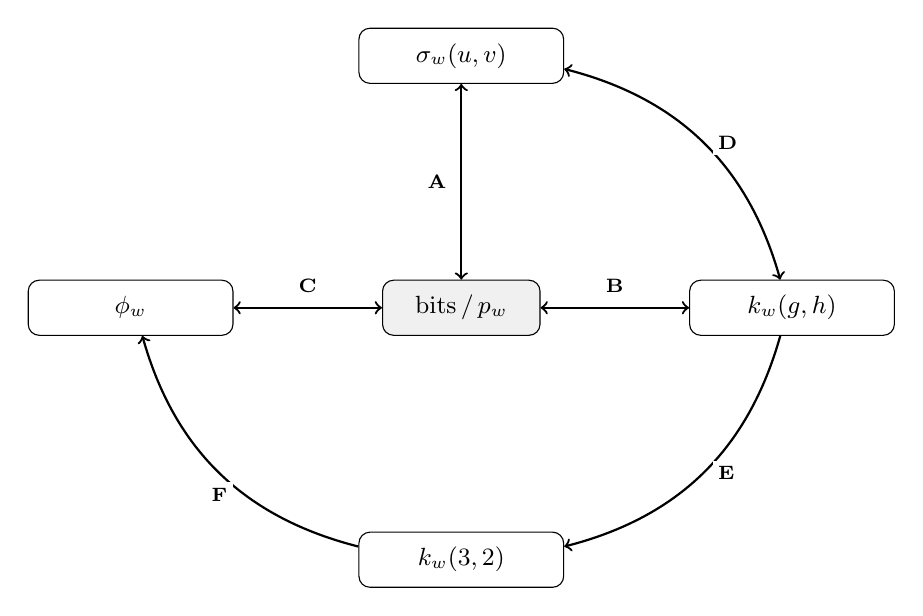
\begin{tikzpicture}[
    nd/.style={draw, rounded corners, fill=white, text centered,
               minimum width=2.6cm, minimum height=0.7cm, font=\small},
    cn/.style={draw, rounded corners, fill=gray!12, text centered,
               minimum width=2.0cm, minimum height=0.7cm, font=\small},
    bi/.style={<->, thick},
    fw/.style={->, thick},
    lbl/.style={font=\scriptsize, fill=white, inner sep=2pt, midway}
  ]
  \node[cn] (bits) at (0, 0)    {bits\,/\,$p_w$};
  \node[nd] (sig)  at (0, 3.2)  {$\sigma_w(u,v)$};
  \node[nd] (kgh)  at (4.2, 0)  {$\kpoly_w(g,h)$};
  \node[nd] (k32)  at (0, -3.2) {$\kpoly_w(3,2)$};
  \node[nd] (phi)  at (-4.2, 0) {$\phi_w$};

  \draw[bi] (bits) -- node[lbl, left=3pt]  {\textbf{A}} (sig);
  \draw[bi] (bits) -- node[lbl, above=3pt] {\textbf{B}} (kgh);
  \draw[bi] (bits) -- node[lbl, above=3pt] {\textbf{C}} (phi);
  \draw[bi] (sig)  to[bend left=30] node[lbl, right=3pt] {\textbf{D}} (kgh);
  \draw[fw] (kgh)  to[bend left=30] node[lbl, right=3pt] {\textbf{E}} (k32);
  \draw[fw] (k32)  to[bend left=30] node[lbl, below=3pt] {\textbf{F}} (phi);
\end{tikzpicture}
\end{center}

\bigskip
\noindent
\begin{tabular}{@{}clp{4.8cm}p{4.4cm}@{}}
\hline
\textbf{Edge} & \textbf{Pair} & \textbf{Forward} & \textbf{Inverse} \\
\hline
\\[-6pt]
\textbf{A} & bits $\leftrightarrow$ $\sigma_w$
  & $\sigma_w(u,v) = \displaystyle\sum_{j=0}^{o-1} u^{o-1-j}\,v^{p_j}$
  & $p_w = \sigma_w(1,2) + 2^n$ \\[10pt]
\textbf{B} & bits $\leftrightarrow$ $\kpoly_w(g,h)$
  & $\kpoly_w(g,h) = \displaystyle\sum_{j=0}^{o-1} g^{o-1-j} h^{\kappa_j}$
  & $p_w = 2^{o-1}\kpoly_w(\tfrac{1}{2},2) + 2^n$ \\[10pt]
\textbf{C} & bits $\leftrightarrow$ $\phi_w$
  & $\phi_w[i] = O$ if $b_i = 1$, else $\phi_w[i] = E$
  & $b_i = 1$ if $\phi_w[i] = O$, else $b_i = 0$ \\[8pt]
\textbf{D} & $\sigma_w \leftrightarrow \kpoly_w(g,h)$
  & $\kpoly_w(g,h) = \sigma_w(gh,h)/h^{o-1}$
  & $\sigma_w(u,v) = \kpoly_w(u/v,\,v)\cdot v^{o-1}$ \\[8pt]
\textbf{E} & $\kpoly_w(g,h) \to \kpoly_w(3,2)$
  & $(g,h)\mapsto(3,2)$
  & (via \textbf{F} then \textbf{C} then \textbf{B}) \\[8pt]
\textbf{F} & $\kpoly_w(3,2) \to \phi_w$ (Def.~\ref{def:phi})
  & $q = 2^e{-}3^o$,\ $a_0 = \kpoly_w(3,2)$;\ iterate $(3,2,q)$ map
  & (via \textbf{C} then \textbf{B}) \\[6pt]
\hline
\end{tabular}

\subsection{The $p$-value (edges B, C; centre node)}

Since $\kpoly_w$ is independent of trailing $E$-steps (Remark~\ref{rem:trailing}),
it does not uniquely identify a parity sequence.  A simple specialisation
recovers a canonical integer encoding, and a sentinel bit resolves the
trailing-$E$ ambiguity.

\begin{proposition}[Bit-encoding of parity sequences]
\label{prop:bits}
Let $w = b_0 b_1 \cdots b_{n-1}$ be a parity sequence of length $n$, where
$b_i = 1$ if the $i$-th step is an $O$-step and $b_i = 0$ if it is an
$E$-step.  Then
\[
  N_w \;:=\; 2^{o-1}\cdot\kpoly_w\!\left(\tfrac{1}{2},\, 2\right)
  \;=\; \sum_{i=0}^{n-1} b_i\, 2^i,
\]
the non-negative integer whose binary representation encodes $w$ directly
(LSB-first, $O = 1$, $E = 0$).
\end{proposition}

\begin{proof}
The $j$-th term of $\kpoly_w(g,h)$ is $g^{o-1-j} h^{\kappa_j}$.  Evaluating
at $g = 1/2$, $h = 2$ and multiplying by $2^{o-1}$:
\[
  2^{o-1} \cdot \left(\tfrac{1}{2}\right)^{o-1-j} \cdot 2^{\kappa_j}
  = 2^{j + \kappa_j}.
\]
Since $\kappa_j$ counts $E$-steps before the $j$-th $O$-step and $j$ counts
$O$-steps before it, $j + \kappa_j = p_j$ is the position of the $j$-th
$O$-step, i.e.\ the index $i$ with $b_i = 1$.  Summing over $j$ gives
$\sum_j 2^{p_j} = \sum_i b_i 2^i = N_w$.
\end{proof}

Sequences differing only in trailing $E$-steps (i.e.\ trailing $b_i = 0$)
share the same $N_w$.  To resolve this ambiguity we append a sentinel bit
at position $n$.

\begin{definition}[$p$-value]
\label{def:pvalue}
The \emph{$p$-value} of a parity sequence $w = b_0 b_1 \cdots b_{n-1}$ is
\[
  p_w \;:=\; \sum_{i=0}^{n-1} b_i\, 2^i \;+\; 2^n
  \;=\; 2^{o-1}\cdot\kpoly_w\!\left(\tfrac{1}{2},2\right) + 2^n.
\]
\end{definition}

\begin{theorem}[$p$-value uniqueness]
\label{thm:pvalue}
The map $w \mapsto p_w$ is a bijection from the set of all finite parity
sequences over $\{O,E\}$ to the set of integers $\geq 2$.  Moreover, $w$ is
uniquely recovered from $p_w$ by writing $p_w$ in binary: the highest set bit
(at position $n$) records the length, and bits $0, \ldots, n-1$ give the
sequence with $1 = O$ and $0 = E$.
\end{theorem}

\begin{proof}
Given $p_w$, let $n = \lfloor \log_2 p_w \rfloor$ (the position of the
highest set bit).  Then bits $0, \ldots, n-1$ of $p_w$ coincide with $N_w$
and uniquely determine the positions of all $O$-steps, hence the full sequence
$w$.  The map is therefore injective.  Surjectivity onto integers $\geq 2$
follows since every such integer has a unique highest set bit at some position
$n \geq 1$, and the lower $n$ bits define a valid parity sequence of length
$n$.
\end{proof}

\subsection{The $\sigma$-polynomial (edges A, D)}

\subsubsection*{Change of variables}

The substitution $g = 1/2$, $h = 2$ that produces $N_w$ can be made
polynomial (avoiding fractional exponents) by a change of variables.

\begin{definition}[$\sigma$-polynomial]
\label{def:sigma}
For a parity sequence $w$ of length $n$ with $o$ odd steps and $O$-step
positions $p_0 < \cdots < p_{o-1}$, define
\[
  \sigma_w(u,v) \;:=\; \kpoly_w\!\left(\tfrac{u}{v},\, v\right) \cdot v^{o-1}
  \;=\; \sum_{j=0}^{o-1} u^{o-1-j}\, v^{p_j}
  \;\in\; \ZZ[u,v].
\]
\end{definition}

The exponent of $u$ in the $j$-th term counts the $O$-steps \emph{after}
position $j$; the exponent of $v$ is the bit-position of the $j$-th $O$-step.
Two specialisations recover the objects already defined:
\[
  \kpoly_w(g,h) \;=\; \frac{\sigma_w(gh,\, h)}{h^{o-1}}, \qquad
  N_w \;=\; \sigma_w(1,\, 2),
\]
and consequently $p_w = \sigma_w(1,2) + 2^n$.

\subsubsection*{The successor operation on $\sigma$}

Each step of the Collatz map acts on $\sigma_w(u,v)$ by an elegant polynomial
operation~\cite{paper14}.  Define
\[
  \gamma_w \;:=\; \begin{cases} 1 & \text{if } p_0 = 0 \text{ (i.e.\ $w$ begins with an $O$-step)}, \\
                                0 & \text{otherwise.} \end{cases}
\tag{$\gamma$}\label{def:gamma}
\]
Equivalently, $\gamma_w = 1$ if and only if the leading term $u^{o-1} v^{p_0}$
of $\sigma_w$ has $v$-exponent zero.  Define
\[
  \operatorname{succ}_\sigma(\sigma_w(u,v))
  \;:=\; u^{\gamma_w} \cdot \sigma_w(u,v) \cdot v^{-1}.
\]
Then $\operatorname{succ}_\sigma(\sigma_w(u,v)) = \sigma_{w'}(u,v)$, where $w'$
is the parity sequence obtained by rotating $w$ left by one step (moving the
first bit to the last position).

\begin{remark}
Adopting the convention $0^0 = 1$, we have $\gamma_w = \sigma_w(1, 0)$:
each term $1^{o-1-j} \cdot 0^{p_j}$ vanishes unless $p_j = 0$, which
occurs precisely when $j = 0$ and $w$ begins with an $O$-step.
\end{remark}

The successor formula is valid in any ring where $u^o = 1$ and $v^n = 1$:
the cycle closes after $n$ steps since $v^{-n} = 1$, returning to $\sigma_w$.
Complex roots of unity are one natural realisation of these constraints, but
the algebraic structure depends only on these two relations.

\subsubsection*{Evaluation at roots of unity}

\begin{proposition}
\label{prop:sigma-roots}
Let $\omega_o = e^{2\pi i/o}$ and $\omega_n = e^{2\pi i/n}$ be primitive
$o$-th and $n$-th roots of unity respectively.  The evaluation
\[
  \sigma_w(\omega_o,\, \omega_n)
  \;=\; \sum_{j=0}^{o-1} \omega_o^{o-1-j}\, \omega_n^{p_j}
\]
expresses the parity sequence as a linear combination of $n$-th roots of
unity, weighted by powers of $\omega_o$.  Each step of the cycle acts as
\[
  \operatorname{succ}_\sigma(\sigma_{w_k}(\omega_o, \omega_n))
  \;=\; \omega_o^{\gamma_{w_k}} \cdot \sigma_{w_k}(\omega_o, \omega_n) \cdot \omega_n^{-1},
\]
a multiplication by $\omega_o^{\gamma_{w_k}}$ (recording whether step $k$ is
an $O$-step) composed with a rotation $\omega_n^{-1}$ of the phase.
Since $\omega_o^o = 1$ and $\omega_n^n = 1$, the cycle closes
after exactly $n$ steps.  See~\cite{paper14} for the full development.
\end{proposition}

\begin{figure}[ht]
\centering
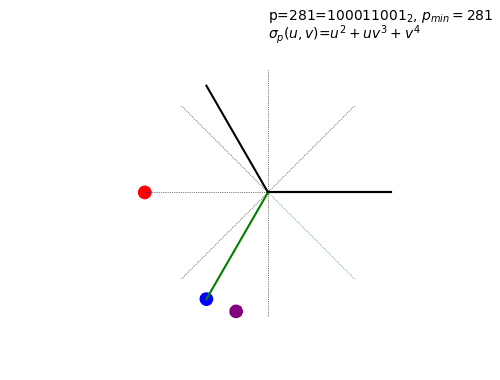
\includegraphics[width=0.32\textwidth]{sigma-frame-0}%
\hfill
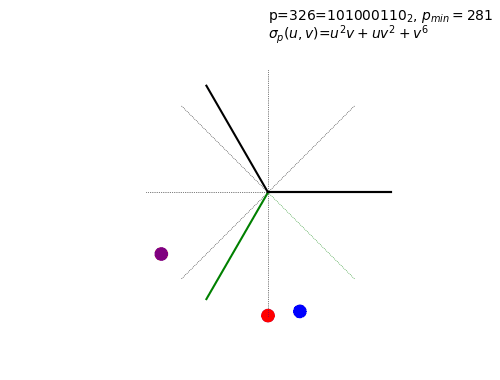
\includegraphics[width=0.32\textwidth]{sigma-frame-2}%
\hfill
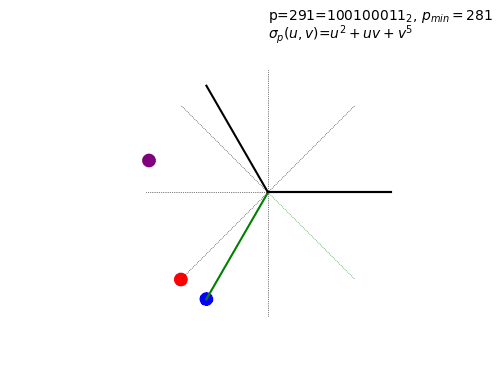
\includegraphics[width=0.32\textwidth]{sigma-frame-3}
\caption{Three successive steps of the $\sigma$-successor for
$w = OEEOEOEE$ ($n=8$, $o=3$), evaluated at $(\omega_3, \omega_8)$.
Coloured dots show the three monomials of $\sigma_w$; the green arrow is
their sum (the value of $\sigma_w$ as a complex number).
\emph{Left} (step~0, $E$-step, $\gamma=0$): $\sigma = u^2 + uv^3 + v^4$.
Notice all three dots rotate together by $\omega_8^{-1}$ — an $E$-step
is a pure phase rotation with no change to the $u$-weights.
\emph{Centre} (after two $E$-steps): $\sigma = u^2 v + uv^2 + v^6$ — the
dots have rotated twice; the sum (green arrow) has changed direction.
\emph{Right} (after the first $O$-step, $\gamma=1$): $\sigma = u^2 + uv + v^5$.
The $O$-step multiplies by $\omega_3$ in addition to rotating by $\omega_8^{-1}$,
redistributing the $u$-weights and visibly changing the triangle of dots.}

\label{fig:sigma-successor}
\end{figure}

\subsection{Worked example (all edges, $w = OEEOEOEE$)}

The remaining nodes $\kpoly_w(3,2)$ and $\phi_w$ are reached via edges E and F
respectively; the return path from $\phi_w$ runs via \textbf{C} then \textbf{B} then \textbf{E}.

\noindent\begin{tabular}{@{}r@{\quad}l@{}}
\textbf{C\textsuperscript{$-1$}} & $b_8 b_7\cdots b_0 = 1,0,0,1,0,1,0,0,1$ \quad ($O{=}1$, $E{=}0$, $b_8{=}1$ sentinel) \\
               & $O$-positions $p_0{=}0,\,p_1{=}3,\,p_2{=}5$ \\[4pt]
\textbf{A}     & $\sigma_w(u,v) = u^2 + u\,v^3 + v^5$ \\
\textbf{A\textsuperscript{$-1$}} & $p_w = \sigma_w(1,2)+2^8 = 41+256 = 297 = 100101001_2$ \\[4pt]
\textbf{D}     & $\kpoly_w(g,h) = \sigma_w(gh,h)/h^2 = g^2+gh^2+h^3$ \\
\textbf{B\textsuperscript{$-1$}} & $p_w = 2^{o-1}\kpoly_w\!\left(\tfrac{1}{2},2\right)+2^8 = 41+256 = 297 = 100101001_2\ \checkmark$ \\[4pt]
\textbf{E}     & $\kpoly_w(3,2) = 3^2+3\cdot 2^2+2^3 = 29$ \\[4pt]
\textbf{F}     & $q=5,\;a_0=29$; iterate $(3,2,5)$: \\
               & $29\xrightarrow{O}92\xrightarrow{E}46\xrightarrow{E}23\xrightarrow{O}
                 74\xrightarrow{E}37\xrightarrow{O}119\xrightarrow{E}62\xrightarrow{E}29
                 \;\Rightarrow\;\phi_w = OEEOEOEE$ \\[4pt]
\textbf{C}     & $b_8 b_7\cdots b_0 = 1,0,0,1,0,1,0,0,1$ \quad($b_8{=}1$ sentinel encodes $n{=}8$) \\
\textbf{B}     & $\kappa_j=(0,2,3)$,\; $\kpoly_w(g,h)=g^2+gh^2+h^3\ \checkmark$
\end{tabular}

\medskip\noindent
Since $\gcd(5,29)=1$, the canonical basis gives $q_w=5$, $a_w=29$:
no $3x{+}1$ cycle, but an integer $3x{+}5$ cycle at $a=29$.

%------------------------------------------------------------
\section{Examples}
\label{sec:examples}
%------------------------------------------------------------

\begin{example}[The $5x+1$ cycle at $17$]
\label{ex:5x1}
Under the Syracuse $5x+1$ map (basis $g = 5$, $h = 2$, $q = 1$), the odd
integer $17$ is a periodic point.  Its orbit is
\[
  17 \;\xrightarrow{O}\; 86 \;\xrightarrow{E}\; 43
     \;\xrightarrow{O}\; 216 \;\xrightarrow{E^3}\; 27
     \;\xrightarrow{O}\; 136 \;\xrightarrow{E^3}\; 17.
\]
The parity sequence is $w = OEOEEEOEEE$, with $o = 3$, $e = 7$.

The $\kappa$-tuple is $\kappa_0 = 0$, $\kappa_1 = 1$, $\kappa_2 = 4$
(the three $O$-steps are preceded by $0$, $1$, and $4$ even steps
respectively).  Note that $(\kappa_0, \kappa_1, \kappa_2) = (0,1,4) \neq
(0,1,2)$, so $w$ is \emph{not} a Steiner word and the geometric polynomial
theorem does not apply directly.  The structural polynomial is
\[
  \kpoly_w(g,h) = g^2 h^0 + g^1 h^1 + g^0 h^4 = g^2 + gh + h^4.
\]
Evaluating at $(g,h) = (5,2)$:
\[
  \kpoly_w(5,2) = 25 + 10 + 16 = 51,
  \qquad
  h^e - g^o = 2^7 - 5^3 = 128 - 125 = 3.
\]
By Theorem~\ref{thm:cycle},
\[
  a = \frac{1 \cdot 51}{3} = 17. \quad \checkmark
\]
The near-miss $h^e - g^o = 3$ is what makes this cycle arithmetically possible:
$2^7 - 5^3 = 3$ is a specific arithmetic accident with no analogue for the
Collatz basis $(g,h) = (3,2)$.  This also illustrates Remark~\ref{rem:pointwise}:
the polynomial $h^7 - g^3$ does not divide $g^2 + gh + h^4$ in $\ZZ[g,h]$,
yet divisibility holds at $(5,2)$ because of this accident.
\end{example}

\begin{example}[The $g = h^2 - 1$ family]
\label{ex:gh2}
When divisibility \emph{does} hold as a polynomial identity, it explains cycles
across an entire family of bases at once.  Consider $\St(1,1)^3$ (three copies
of $OEE$), with $o = 3$, $e = 6$.  By the composition rule:
\begin{align*}
  \kpoly_{\St(1,1)^2}(g,h) &= g + h^2, \\
  \kpoly_{\St(1,1)^3}(g,h) &= g^2 + gh^2 + h^4.
\end{align*}
On the locus $g = h^2 - 1$ one checks that $(g^2 + gh^2 + h^4) - (h^6 - g^3)
= (g - h^2 + 1)(g^2 + gh^2 + h^4)$ vanishes identically on the locus $g = h^2-1$
(since $g - h^2 + 1 = 0$ there), so
$\kpoly_{\St(1,1)^3} = h^6 - g^3$ and the cycle element
$a = q\cdot\kpoly/(h^6-g^3) = q$ for every such basis.  At $q=1$:
\begin{itemize}
  \item $h=2$, $g=3$: orbit $1\xrightarrow{O}4\xrightarrow{EE}1$, three times.
  \item $h=3$, $g=8$: orbit $1\xrightarrow{O}9\xrightarrow{EE}1$, three times.
\end{itemize}
\end{example}

\begin{example}[Non-Collatz parity sequence]
\label{ex:noncollatz}
This example relaxes the requirement that the $\kappa$-tuple be strictly
increasing.  In the integer domain this corresponds to relaxing the rule
that $gx+q$ is applied only to odd integers; in both settings the result
is an ``illegal'' cycle that does not arise in standard Collatz dynamics.

Consider the parity sequence $w = OEEOOEEE$, with $o = 3$, $e = 5$.
The $\kappa$-tuple is $\kappa_0 = 0$, $\kappa_1 = 2$, $\kappa_2 = 2$:
both the second and third $O$-steps are preceded by exactly 2 even steps.
The structural polynomial is
\[
  \kpoly_{OEEOOEEE}(g,h)
    = g^{2}h^{0} + g^{1}h^{2} + g^{0}h^{2}
    = g^2 + h^2(g + 1).
\]

This $w$ is \emph{not} a valid standard Collatz parity sequence.
The equal values $\kappa_1 = \kappa_2 = 2$ mean that two consecutive $O$-steps
occur without any intervening $E$-step---the subsequence $OO$ appears.
Under standard Collatz, an $O$-step must be applied to an odd integer, so
two consecutive $O$-steps are impossible: after $3n+1$ the result is even
and must be halved before another $O$-step can occur.  Equivalently, valid
Collatz sequences require $\kappa_0 < \kappa_1 < \cdots < \kappa_{o-1}$
(strictly increasing).

If one relaxes this single condition---allowing $\kappa_j \le \kappa_{j+1}$---and
correspondingly drives the $3x+1$ and $x/2$ operations by the letters of $w$
rather than the parity of the current element, then cycles can exist.  At
$(g,h) = (3,2)$ we get $\kpoly_w(3,2) = 3^2 + 2^2(3+1) = 9 + 16 = 25$ and
$h^e - g^o = 2^5 - 3^3 = 5$, so Theorem~\ref{thm:cycle} yields cycle element
$a = 25/5 = 5$.  The orbit from $a = 5$ is
\[
  5 \xrightarrow{O} 16 \xrightarrow{E} 8 \xrightarrow{E} 4
    \xrightarrow{O} 13 \xrightarrow{O} 40 \xrightarrow{E} 20
    \xrightarrow{E} 10 \xrightarrow{E} 5,
\]
which does return to $5$.  The single illegal step is $4 \xrightarrow{O} 13$:
applying $3x+1$ to the even integer $4$, forced by the repeated value
$\kappa_1 = \kappa_2 = 2$.
\end{example}

\begin{remark}
The sequence $OEEOOEEE$ above has $p$-value $N_w + 2^8 = 25 + 256 = 281$:
the integer $281$ encodes the sequence directly in binary (with sentinel bit
at position $8$), and the glitched orbit was constructed by reading the bits
of $281 - 256 = 25$ as a parity sequence.
\end{remark}

%------------------------------------------------------------
\section{Related Work}
\label{sec:related}
%------------------------------------------------------------

The structural polynomial $\kpoly_w(g,h)$ is closely related to the
$k$-parameter appearing in the standard affine representation of Collatz
orbits, where it appears as an entry in the affine transformation matrix.
The Steiner word framework was developed
in~\cite{paper67} as a natural decomposition of Syracuse orbits; the present
paper provides its polynomial algebraic foundation.

The $\sigma$-polynomial $\sigma_w(u,v)$ and its successor operation at complex
roots of unity were introduced in~\cite{paper14}; the present paper situates
them within the broader five-representation framework and makes their
connection to $\kpoly_w(g,h)$ via the change of variables $g = u/v$, $h = v$
explicit.

The composition rule (Theorem~\ref{thm:composition}) and cycle element identity
(Theorem~\ref{thm:cycle}) are applied in the companion paper~\cite{paper73} to
prove a uniqueness theorem for the $2a+1$ Steiner composition identity and to
characterise its domain constraint in terms of $2$-adic valuations.
Structural constraints on Collatz cycles derived from Steiner sentence analysis
appear in~\cite{paper68}.

%------------------------------------------------------------
\begin{thebibliography}{99}

\bibitem{paper14}
J.\ Seymour,
\textit{Exploring Cyclic Structures in Polynomial Rings with Applications to the Collatz Conjecture},
preprint, 2025.
\url{https://wildducktheories.github.io/collatz/papers/14-uv-polynomial/uv-polynomial.pdf}

\bibitem{paper67}
J.\ Seymour,
\textit{Steiner Word Decomposition and Branch Length Distribution},
preprint, 2026.
\url{https://wildducktheories.github.io/collatz/papers/67-branch-length-distribution/67-branch-length-distribution.pdf}

\bibitem{paper68}
J.\ Seymour,
\textit{Structural Constraints on Collatz Cycles via Steiner Sentence Analysis},
unpublished, 2026.

\bibitem{paper73}
J.\ Seymour,
\textit{The $2a+1$ Composition Identity: Uniqueness and Domain Constraint},
unpublished, 2026.

\end{thebibliography}

\end{document}
